\documentclass{article}
\usepackage[main=spanish,activeacute,spanish]{babel}
\usepackage[utf8]{inputenc}
\usepackage{graphicx} 
\usepackage{ragged2e}
\usepackage{subfig}
\usepackage[utf8]{inputenc}
\usepackage{float}
\usepackage{amsmath}
\usepackage{tikz-cd}
\usepackage{amssymb}
\usepackage{enumerate}
\usepackage{mathtools}
\usepackage{hyperref}

\newcommand{\norm}[1]{\left\lVert#1\right\rVert}

\title{Transferencia de momento lineal en dos dimensiones}


\author{Carlos A. Toro, Lucas H. Quiceno, Victor M. Oviedo}
\date{Agosto 2021}

\begin{document}

\maketitle
\begin{abstract}
    A continuación presentamos la física que está por detrás del juego de billar, esto es, la física de las colisiones entre varios cuerpos y en diversas circunstancias. El concepto físico crucial para entender estos fenómenos es el del momento lineal, el cual abordaremos desde dos perspectivas. Inicialmente consideramos una explicación para estudiantes que aún no han tenido contacto con herramientas muy útiles de las matemáticas como es el cálculo diferencial. Luego desarrollamos una sección orientada para estudiantes más avanzados, la cual tiene un sabor mucho más matemático y formal, pero que discute los mismos temas que se abordaron en la sección para principiantes. Finalmente en la última sección mostramos los cálculos matemáticos que se necesitaron para crear la simulación de la mesa de billar.
\end{abstract}

\section{Explicación principiantes}
Las leyes de Newton que comúnmente se enseñan en todos los colegios desde temprana edad, son un marco teórico y conceptual muy importante que permite solucionar problemas de la vida cotidiana, tales como el movimiento de un auto o un cohete. Nos dice como cae un cuerpo que se libera en el aire, estas leyes se pueden aplicar en un sin fin de situaciones de la vida diaria.

Sin embargo, el estudiante curioso, quizás cuando juega a los “balines” con sus amigos, se hace la siguiente pregunta: ¿cómo deciden dos balines cuando chocan para que lado dirigirse luego del choque?. Al pasar los días, el mismo estudiante curioso se da cuenta que cuando los balines chocan interaccionan por un tiempo muy corto y además, nota que puede encontrar situaciones que se asemejan a la de los balines, como lo  son, los choques entre dos autos, el choque cuando un bate golpea la bola jugando béisbol, o en un simple juego de billar.

Las situaciones descritas anteriormente llevan al estudiante curioso a descubrir que existen nuevos conceptos más allá de las leyes de Newton que le permiten estudiar estas situaciones, el estudiante se encuentra con que hay cantidades que se conservan como los son la energía o el momento lineal y que con estos nuevos conceptos puede estudiar situaciones más amplias como el comportamiento del núcleo atómico y los electrones.

\subsection{Momento lineal}
Desde la física, cuando se quiere estudiar la colisión de dos objetos, como bolas de billar, una cantidad física importante a considerar es el momento lineal, pues da información acerca de la velocidad a la que van los objetos pero también nos habla sobre cuanta masa tiene cada objeto. Tanto la velocidad como la masa son valores que determinan el comportamiento antes y después de cada colisión.

\subsection{Impulso}
Dado que todo evoluciona con el tiempo, es importante ver como las cantidades físicas cambian con el tiempo. Una herramienta matemática muy útil para estudiar estos cambios son las derivadas. Una derivada nos da cuenta del cambio de una cantidad respecto a otra, por ejemplo, una fuerza es el cambio del momento respecto al tiempo (la derivada del momento respecto al tiempo). Con lo anterior, se puede definir el impulso que se le da a un objeto como la fuerza que actúa durante cierto intervalo de tiempo.

\subsection{Conservación del momento lineal}
Cantidades como el momento lineal y la energía están sujetas a leyes de conservación. Por ejemplo, en un sistema (como un par de bolas en nuestra mesa de billar) donde no hay fuerzas externas (como el golpe que un jugador de billar le da a las bolas o la fricción entre el aire y cada bola) o donde todas las fuerzas se anulan entre si, la suma del momento lineal de todas las bolas no cambiará con el tiempo, es decir, es un valor que permanece constante.

\subsection{Choques}

Todos los conceptos que hemos mencionado nos traen de vuelta al primer problema con el que el estudiante se encontró al principio, ¿cómo chocan dos bolas en un corto periodo de tiempo pero que llevan una gran fuerza de impacto?

\subsubsection{Choque elástico}

Podemos clasificar los choques usando la energía y las leyes de conservación como criterio, así, un choque elástico es aquel  en el que no hay ni perdida ni ganancia de energía, es decir, la energía se conserva. En el caso del billar, si ignoramos la pérdida de energía por la fricción sobre las bolas, se puede decir que el choque es elástico. Esto no es exactamente lo que sucede en realidad, pero es una buena forma de dar un primer acercamiento al estudio del problema de las colisiones.

\subsubsection{Choques inelásticos}
Cuando nos referimos a energía cinética estamos hablando de la energía que tiene un objeto por el hecho de estar en movimiento.
Se dice que un choque es inelástico cuando la energía  cinética final es menor que la energía cinética inicial. Al igual que el momento lineal, la energía cinética también depende de que tanta masa tenga un objeto y de la velocidad que lleve. Entonces en un choque inelástico las partículas pierden algo de su masa, algo de su velocidad o ambas. Un ejemplo particular es cuando se dispara una bala hacía una persona, esta se incrustra y no hay rebote, la bala y la persona pasan a considerarse como un mismo cuerpo.

\section{Explicación avanzada}
\subsection{Momento lineal}
De la segunda ley de Newton [1] en forma vectorial, $\textbf{F}=\frac{d\textbf{p}}{dt}$ se puede escrbir en la siguiente forma, considerando a la masa $m$ constante,

\begin{equation}
   \textbf{F}=\frac{d\textbf{p}}{dt}=\frac{d(m\textbf{v})}{dt}=m\frac{d\textbf{v}}{dt}=m\textbf{a}
\end{equation}

La cantidad entre paréntesis es espacial en física y recibe el nombre del momento lineal, definido como

\begin{equation}
   \textbf{p}=m\textbf{v}
\end{equation}

Expresando la anterior ecuación en sus componentes en un movimiento en dos dimensiones se obtiene

\begin{equation}
   \textbf{p}_{x}=m\textbf{v}_{x}
\end{equation}

\begin{equation}
   \textbf{p}_{y}=m\textbf{v}_{y}
\end{equation}

\subsection{Impulso}

La energía cinética se define como $\frac{1}{2}mv^{2}$, estamos interesados en ver la diferencia de esta cantidad con el momento, para ello consideremos una fuerza que actúa en un intervalo de tiempo $t_{1}$ a  $t_{2}$  y definimos el impuslo como

\begin{equation}
   \textbf{J}=\textbf{F} (t_{2}-t_{1}) = \textbf{F}\delta t
\end{equation}

Será de interés el teorema del impulso y el momento lineal que relaciona esta cantidades

\begin{equation}
   \textbf{J}=\textbf{p}_{1} - \textbf{p}_{2}
\end{equation}

En palabras se puede expresar diciendo que el cambio en el momento lineal de una partícula es igual al impulso que genera una fuerza en ese intervalo de tiempo.

\subsection{Conservación del momento lineal}

La conservación del momento lineal es importante cuando se tienen sistemas de más de dos partículas que interactúan entre si, por ejemplo, si se tiene un sistema de una sola partícula no es común escuchar la conservación del momento lineal. Cuando el número de partícula aumenta si es común que entre las cantidades conservadas se encuentre el momento lineal, que en palabras se enuncia así: si la suma vectorial de todas las fuerzas que actúa en un sistema de muchas partículas es cero, entonces el momento lineal total es constante. Esto nos dice que si tenemos un sistema que cumple la condición anterior y conocemos su momento lineal inicial, este será igual a su momento lineal final.

\subsection{Choques}

Todos los conceptos que hemos estudiado nos traen de vuelta al primer problema con el que el estudiante se encontró al principio, ¿cómo chocan dos bolas en un corto periodo de tiempo pero que llevan una gran fuerza de impacto?

\subsubsection{Choque elástico}

Un choque elástico es aquel en el que las fuerzas que actúan son conservativas, esto quiere decir que durante el choque, durante la interacción, no hay perdida de energía pero, tampoco hay ganancia de energía, es decir, la energía se conserva, un ejemplo de un choque elástico es el choque de dos bolas de billar, obviamente hay un pérdida de energía por fricción, pero esta pérdida es tan pequeña que se puede despreciar completamente y suponer que este tiempo de choques son completamente elásticos.

Cuando ocurre un choque elástico, imagine dos bolas de billar durante el periodo que éstas se encuentran en contacto, ocurren pequeñas deformaciones sobretodo a nivel atómico pero luego se restablece a la forma que tenían antes del choque.

Supongamos dos bolas, una con  masa $m_{A}$ y velocidad  $\textbf{v}_{A}$ y otra con masa $m_{B}$ y velocidad  $\textbf{v}_{B}$ que chocan. Usando la conservación de la energía se obtiene

\begin{equation}
   \frac{1}{2} m_{A} \textbf{v}_{A1}^{2}+  \frac{1}{2} m_{B} \textbf{v}_{B1}^{2} = \frac{1}{2} m_{A}  \textbf{v}_{A2}^{2}+ \frac{1}{2} m_{B} \textbf{v}_{B2}^{2}
\end{equation}


y usando la conservación del momento lineal obtenemos

\begin{equation}
  m_{A} \textbf{v}_{A1} + m_{B} \textbf{v}_{B1} = m_{A} \textbf{v}_{A2} + m_{B} \textbf{v}_{B2}
\end{equation}

es decir, si medimos las masas y las velocidades iniciales podemos, despejando de estas ecuaciones, obtener las velocidades finales.

\subsubsection{Choques inelásticos}
Se dice que un choque es inelástico cuando la energía  cinética final es menor que la energía cinética inicial, un ejemplo particular es cuando se dispara una bala hacía una persona, esta se incrustra y no hay rebote, la bala y la persona pasan a considerarse como un mismo cuerpo.

Usemos las conservación de la energía y del momento lineal para ver qué sucede en un choque totalmente inelástico. Supongamos dos cuerpos, uno con velocidad $\textbf{v}_{A}$  y otro con velocidad $\textbf{v}_{B}$ que chocan y pasan a ser uno solo, después del choque quedan con la misma velocidad que se puede representar por la ecuación  

\begin{equation}
   \textbf{v}_{A2}=\textbf{v}_{B2} = \textbf{v}_{2}
\end{equation}

Usando la conservación del momento lineal se obtiene

\begin{equation}
  m_{A} \textbf{v}_{A1} + m_{B} \textbf{v}_{B1} = (m_{A} + m_{B})\textbf{v}_{2}
\end{equation}

La anterior ecuación nos dice que si podemos medir la masa y las velocidades iniciales de las partículas podemos conocer la velocidad del cuerpo .


\section{Simulación}

En la presente simulación, se analizará la colisión entre $N$ bolas de billar rígidas. A continuación se aplicarán los conceptos discutidos en el marco teórico para considerar el caso particular de un choque entre dos de estas bolas de billar y que fue implementado en la simulación desarrollada.

\subsection{Análisis sin medio viscoso}
Con referencia a la Figura 1, supóngase que inicialmente en el vacío se tienen dos bolas de billar de masas $m_1$ y $m_2$ con velocidades $\textbf{v}_{i}$ y $\textbf{w}_{i}$ respectivamente, colisionan durante un tiempo infinitesimal $\delta t$ interactuando por medio de una fuerza interna central $\textbf{F}$ para después moverse con velocidades finales $\textbf{v}_{f}$ y $\textbf{w}_{f}$.

\begin{figure}[h]
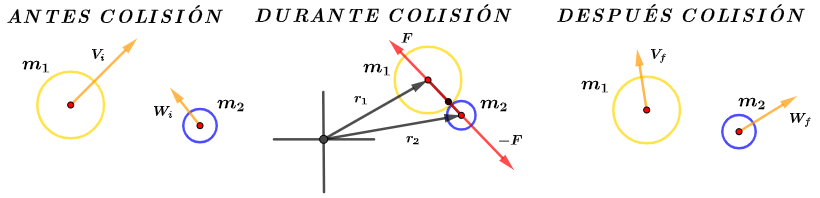
\includegraphics[width=\linewidth]{colision.png}
\caption{Choque de dos bolas de billar.}
\end{figure}

Adicionalmente, se asume que las fuerzas externas al sistema formado por las dos bolas son exactamente cero y por lo tanto el momento total se conserva.\\\\La conservación del momento viene dada por la siguiente ecuación
\begin{equation}
    m_1\textbf{v}_{i}+m_2\textbf{w}_{i}=m_1\textbf{v}_{f}+m_2\textbf{w}_{f}.
\end{equation}
En términos del cambio de momento $\Delta p$ de cada partícula y teniendo en cuenta la definición de impulso dada en la ecuación (5) podemos escribir la ecuación (11) como

\begin{equation}
    \Delta \textbf{p}_{1}=-\Delta \textbf{p}_{2}=\textbf{F}\delta t.
\end{equation}

Como la fuerza $\textbf{F}$ es central, podemos representarla de la siguiente forma

\begin{equation}
    \textbf{F}\delta t=\norm{\textbf{F}}\delta t\frac{\textbf{r}_{1}-\textbf{r}_{2}}{\norm{\textbf{r}_{1}-\textbf{r}_{2}}}=a\hat{\textbf{u}}
\end{equation}

donde hemos definido el vector unitario $\hat{u}=\frac{\textbf{r}_{1}-\textbf{r}_{2}}{\norm{\textbf{r}_{1}-\textbf{r}_{2}}}$ y el parámetro $a=\norm{\textbf{F}}\delta t$. En términos de estas cantidades $\hat{\textbf{{u}}}$ y $a$, con ayuda de la ecuación (12) podemos calcular las velocidades finales de ambas bolas

\begin{gather}
    \textbf{v}_{f}=\textbf{v}_{i}+\frac{a}{m_1}\hat{\textbf{u}} \\ 
    \textbf{w}_{f}=\textbf{w}_{i}-\frac{a}{m_2}\hat{\textbf{u}}.
\end{gather}

Note que el vector unitario $\hat{\textbf{u}}$ es posible calcularlo en términos de los vectores posición $\vec{r_1}$ y $\vec{r_2}$, sin embargo el parámetro $a$ debe calcularse a partir de condiciones sobre el tipo de choque, por ejemplo si el choque es completamente elástico, completamente inelástico o un caso intermedio entre estos extremos. Antes de proseguir con el caso general, analicemos el ejemplo de un choque completamente elástico en donde hay conservación de la energía cinética.
\subsubsection{Caso completamente elástico}

En un choque elástico tenemos de (7) que
\begin{equation}
    \frac{1}{2} m_1 v_i^2+   \frac{1}{2} m_2 w_i^2 =  \frac{1}{2} m_1 v_f^2+  \frac{1}{2} m_2 w_f^2
\end{equation}
 reemplazando las ecuaciones (14) y (15) en (16) y realizando un poco de álgebra elemental, se obtiene la siguiente solución física para $a$ [2]
 \begin{equation}
     a= \frac{2m_1m_2}{m1+m_2}((\textbf{w}_{i}-\textbf{v}_{i})\cdot \hat{\textbf{u}})
 \end{equation}


\subsubsection{Caso general}
Regresando al caso general, en el cual es posible tener un choque entre los extremos inelásticos y elásticos, se cuenta con un coeficiente que es útil para caracterizar los distintos tipos de colisiones, este es el coeficiente de restitución $k$ dado por la siguiente ecuación

\begin{equation}
    k=\frac{\norm{\textbf{v}_{f}-\textbf{w}_{f}}}{\norm{\textbf{v}_{i}-\textbf{w}_{i}}}
\end{equation}

reemplazando las ecuaciones (14) y (15) en (18) podemos expresar el coeficiente de restitución en terminos del parámetro $a$ de la siguiente forma

\begin{equation}
    k=\frac{\norm{\textbf{v}_{i}-\textbf{w}_{i}+a(\frac{1}{m_1}+\frac{1}{m_2})\hat{\textbf{u}}}}{\norm{\textbf{v}_{i}-\textbf{w}_{i}}}
\end{equation}

elevando al cuadrado ambos miembros y multiplicando ambos lados por el factor $|\textbf{v}_{i}-\textbf{w}_{i}|^2$ se obtiene la siguiente ecuación de segundo grado en $a$

\begin{equation}
    \left(\frac{1}{m_1}+\frac{1}{m_2}\right)^2a^2+2\left(\frac{1}{m_1}+\frac{1}{m_2}\right)((\textbf{v}_{i}-\textbf{w}_{i})\cdot \hat{\textbf{u}})a+(1-k^2)\norm{\textbf{v}_{i}-\textbf{w}_{i}}^2=0.
\end{equation}

Nótese que por la ecuación (9), un choque completamente inelástico está caracterizado por que las velocidades finales $\textbf{v}_{f}$ y $\textbf{w}_{f}$ son iguales, lo que implica de (18) que el coeficiente de restitución $k$ es nulo. Por tanto la condición $k=0$ caracteriza los choques completamente inelásticos. Se demostrará ahora que la condición $k=1$ caracteriza los choques completamente elásticos.\\\\En efecto reemplazando en (20) la solución encontrada de $a$ en (17) para el caso totalmente elástico, se deduce que $(1-k^2)\norm{\textbf{v}_{i}-\textbf{w}_{i}}^2=0$, de donde se concluye que $k=1$ desde que $k\geq 0$ por la misma definición del coeficiente de restitución. Por tanto la condición $k=1$ caracteriza los choques completamente elásticos como se quería mostrar.\\\\ En la práctica, es decir en la simulación, se parte de un coeficiente de restitución conocido y dado por el usuario, generalmente entre $0$ y $1$, el cual se ingresa en la ecuación (20) como valor de entrada y se determina la solución positiva para $a$ de dicha ecuación de segundo grado. Una vez determinado el valor de $a$ a partir del coeficiente de restitución y de las masas, posiciones y velocidades iniciales  de las bolas de billar, se procede a reemplazarlo en las ecuaciones (14) y (15) para hallar las velocidades finales.\\\\
Una observación importante con respecto al coeficiente de restitución en una determinada colisión, es que para obtener soluciones reales de $a$ a partir de la ecuación (20), debe existir un valor mínimo $k_{min}$ de dicho coeficiente, se procede a continuación a estimar dicho valor mínimo. En efecto, analizando el discriminante $D$ de la ecuación cuadrática (20) se sigue que para obtener soluciones reales se debe cumplir que $D\geq0$, luego

\begin{equation}
   0\leq D = 4\left(\frac{1}{m_1}+\frac{1}{m_2}\right)^2(\textbf{v}_{i}-\textbf{w}_{i})\cdot \hat{\textbf{u}})^2- 4\left(\frac{1}{m_1}+\frac{1}{m_2}\right)^2(1-k^2)^2\norm{\textbf{v}_{i}-\textbf{w}_{i}}^2.
\end{equation}

 definiendo un vector unitario $\hat{\textbf{s}}=\frac{\textbf{v}_{i}-\textbf{w}_{i}}{\norm{\textbf{v}_{i}-\textbf{w}_{i}}}$, similar al vector unitario $\hat{\textbf{u}}$ y solucionando la desigualdad (21) se obtiene el valor mínimo para el coeficiente de restitución 
 \begin{equation}
     k\geq \sqrt{1-\norm{\hat{\textbf{s}}\cdot \hat{\textbf{u}}}^2}:=k_{min}
 \end{equation}
 
 Note que la raíz cuadrada en la ecuación (22) está bien definida ya que como los vectores $\hat{\textbf{s}}$ y $\hat{\textbf{u}}$ son unitarios y por la desigualdad de Cauchy-Schwarz $\norm{\hat{\textbf{s}}\cdot \hat{\textbf{u}}}\leq \norm{\hat{\textbf{s}}}\norm{\hat{\textbf{u}}}=1$ se sigue que $1-\norm{\hat{\textbf{s}}\cdot \hat{\textbf{u}}}^2\geq 0$.
 
 \subsection{Análisis con medio viscoso}
 
 Consideramos de nuevo la colisión entre dos bolas de billar, como en la Figura 1, pero esta vez, suponiendo que se encuentran sumergidas en un medio viscoso, puede ser aire, agua, aceite o algún material que produzca resistencia al movimiento de dichas bolas. Se modelará esta fuerza de fricción $\textbf{$F_r$}$ como proporcional a la velocidad $\textbf{v}$ de la bola y en sentido contrario. Para simplificar los cálculos no se tendrá en cuenta la geometría de las bolas, es decir, la fuerza de fricción actuará sobre objetos puntuales. LLamando $b$ al coeficiente de proporcionalidad entre la fuerza de fricción y la velocidad, el cual es un parámetro que el usuario deberá ingresar, se tiene que $ \textbf{$F_r$}= -b \textbf{v}$ [1].\\
 
 La segunda ley de Newton toma la forma
 
 \begin{equation}
 \textbf{$F_r$}= -b \textbf{v} = m \frac{d  \textbf{v}}{dt}
 \end{equation}
 
 solucionando para la velocidad se tiene
 
 \begin{equation}
 \textbf{v} =  \textbf{v}_{0} e^{- \frac{bt}{m}}
 \end{equation}
 
 de donde se sigue que si $b=0$, es decir, no hay fricción, se recupera la expresión de un movimiento libre.
 
 Debido a la fuerza de fricción, el sistema ya no es un sistema aislado donde las fuerzas externas son nulas y por tanto la conservación del momento no es válida. Sin embargo, se puede suponer que el momento lineal se conserva durante el instante inmediatamente anterior a la colisión y el instante posterior a ella, para que sea válida la ecuación (12) y poder calcular las velocidades después de la colisión. 










\section{Referencias}
[1] Young, Hugo D. y Freedman, Roger A. Física Universitaria Vol. I, Decimosegunda edición, PEARSON EDUCACÍON, 2009.

[2] https://www.sjsu.edu/faculty/watkins/collision.htm


\end{document}

